\documentclass{article}
\usepackage{graphicx}
\usepackage{hyperref}
\usepackage{multirow}

\begin{document}

\title{Project 3}
\author{Jake Carlson}
\date{November 4, 2017}
\maketitle

\abstract
This report examines federal payroll data in the years 2005 and 2013. The data will be transformed into transaction data so that association rule mining can be performed. By looking at the differences in maximal, closed, and frequent itemsets, I will be able to understand common features about employees under the presidencies of George W. Bush and Barack Obama.

\newpage

\tableofcontents
\newpage

\section{Business Understanding}
In this report I will again be examining the federal payroll data obtained by BuzzFeed News through the Freedom of Information Act. I will look at the years 2005 and 2013 so I can gauge how the government changed as the presidency transitioned from George W. Bush to Barack Obama. This report will focus on association rule mining. The payroll data will be formatted as transaction data, where each employee is treated as a bag of features where all attributes that apply to them are placed in their bag. With the data formatted in this way, I can use the arules package to find items that occur together. These items can be treated as rules, where the occurance of some items tend to imply the occurance of another item. With these rules, along with statistics about the rule such as the support, or the ratio of instances that express the rule, and confidence, or the conditional probability that the predicted item occurs in an instance which contains all remaining items for the rule, I will build a picture of the key differences between groups of federal employees under the two presidents.

\section{Data Preparation}
I will start with the data as I prepared it for classification in Project 2. This data has been cleaned such that all unknown values were replaced with NA, Age and Length of Service were adjusted to take the middle year for the range of years given in the raw data, and Pay has ben discretized into the pay ranges given in Table \ref{tab:1}. In addition, Education is descritized into the groups given in Table \ref{tab:2}.
\par
I will get rid of attributes that I am not interested in for association rule mining. I will drop the Agency attribute because AgencyName already encodes this data. Likewise, I will drop Station because region records the state an employee works in.
\par
All numeric fields will be discretized based on frequency **explain why**. SupervisoryStatus must be treated as a factor so that general employees are not grouped with supervisors. The final list of attributes is given in Table \ref{tab:3}.
\par
These attributes are then transformed into a transaction item matrix. The most frequent items show us what attributes are the most common for employees to have. Summaries for both the 2005 and 2013 transaction data sets are given in Table \ref{tab:4}. We see that for both years, the most common employees are non-supervisors. The majority of employees are also college educated and have been working in the federal government for less than twelve years. Most employees are younger than 47 years old and the most frequent employment category is Administrative.

    \begin{center}
        \begin{table}
            \centering
            \begin{tabular}{ |c| }
                \hline
                Pay Ranges \\
                \hline
                $<$30k \\
                30-50k \\
                50-70k \\
                70-90k \\
                90-110k \\
                $>$110k \\
                \hline
            \end{tabular}
            \caption{The Pay Ranges Used To Descretize Pay}
            \label{tab:1}
        \end{table}
    \end{center}

    \begin{center}
        \begin{table}
            \centering
            \begin{tabular}{ |c|c|c| }
                \hline
                Group & Education Levels & Description \\
                \hline
                Elm & 0, 1 & Reached or completed elementary school \\
                HS & 3, 4, 5, 6 & Reached or completed high school or an occupational program \\
                Col & 7, 8, 9, 10, 11, 12, 13 & Reached or completed college with a Bachelor's degree \\
                Grad & 14, 15, 16, 17, 18, 19, 20 & Any level of graduate studies, excluding a Doctorate \\
                Doc & 21, 22 & A Doctorate or Post-Doctorate degree \\
                \hline
            \end{tabular}
            \caption{Ordinal Education Groups}
            \label{tab:2}
        \end{table}
    \end{center}

    \begin{center}
        \begin{table}
            \centering
            \begin{tabular}{ |c|c|c| }
                \hline
                Attribute & Scale & Range \\
                \hline
                AgencyName & Nominal & The name of each agency \\
                region & Nominal & The name of the state \\
                Age & Interval & [17,47), [47,57), [57,75] \\
                Education & Ordinal & Elm, HS, Col, Grad, Doc \\
                LOS & Interval & [1,22), 22, [27,35] \\
                Category & Nominal & P, A, T, C, O, B \\
                Pay & Ordinal & $<$30k, 30-50k, 50-70k, 70-90k, 90-110k, $>$110k \\
                SupervisoryStatus & Nominal & 2, 4, 5, 6, 7, 8 \\
                \hline
            \end{tabular}
            \caption{Final Data Set Attributes}
            \label{tab:3}
        \end{table}
    \end{center}

    \begin{center}
        \begin{table}
            \centering
            \begin{tabular}{ |c|c|c| }
                \hline
                \multirow{8}{*}{2005} & Elements & 4,720,680 \\
                \cline{2-3}
                & Item & Count \\
                \cline{2-3}
                & SupervisoryStatus=8 & 4,081,468 \\
                & Education=Col & 2,190,442 \\
                & Age=[17,47) & 2,087,004 \\
                & LOS=[1,12) & 1,900,001 \\
                & Category=A & 1,716,162 \\
                \cline{2-3}
                & Itemset Length & Count \\
                \cline{2-3}
                & 4 & 18 \\
                & 5 & 2529 \\
                & 6 & 85,052 \\
                & 7 & 2,034,281 \\
                & 8 & 2,598,800 \\
                \hline
                \multirow{8}{*}{2013} & Elements & 5,323,899 \\
                \cline{2-3}
                & Item & Count \\
                \cline{2-3}
                & SupervisoryStatus=8 & 4,502,511 \\
                & Education=Col & 2,574,899 \\
                & LOS=[1,12) & 2,568,556 \\
                & Age=[17,47) & 2,276,609 \\
                & Category=A & 2,034,255 \\
                \cline{2-3}
                & Itemset Length & Count \\
                \cline{2-3}
                & 5 & 126 \\
                & 6 & 13,770 \\
                & 7 & 2,173,306 \\
                & 8 & 3,136,697 \\
                \hline
            \end{tabular}
            \caption{Summaries of 2005 and 2013 Transaction Data Sets}
            \label{tab:4}
        \end{table}
    \end{center}

\section{Modeling}
In order to mine the transaction data for meaningful rules, I will examine frequent, closed, and maximal itemsets.

    \subsection{Frequent Itemsets}
    The most frequent itemsets show the attributes that are shared by the most number of employees. The most frequent itemsets have the highest support value out of all of the itemsets. I will look for itemsets that occur for 1\% of all employees. It is also useful to view itemsets with more items to see what attributes occur frequently together. The distribution of itemset sizes is given in Figure \ref{fig:1}. We see that the distribution of sizes is consistent between the two years.
    \par
    In order to gauge differences between the two administrations, I will examine the most frequent itemsets which contain more than five items. The relative item frequency for items in itemsets with length six are given in Figure \ref{fig:2} for 2005 and Figure \ref{fig:3} for 2013.
    \par
    A number of trends are apparent in these graphs. We see an increase in the ratio of employees who have a Graduate level education, as well as a reduction in the ratio of employees who have a High School level education under the Obama administration.  Also, there is a decrease in the ratio of employees who have a Length of Service between 12 and 22 years, with an increase in employees who have worked for the government for less than 12 years. This is consistent with Project 1 where I found that Obama employed newer employees, while employees hired before the Bush administration looked for employment elsewhere \cite{proj1}.
    \par
    Another noticable trend is the frequency of employees who worked for the Transportation Security Administration. Under Bush, the number of employees in the TSA is quite large, reflecting the growth of the agency in response to the September 11th attacks. The TSA shrunk in size relative to the VHA under Obama. This reflects the growth of the Veterans Affairs Administration under the Obama administration.
    \par
    To look closer at the relationships between items in these itemsets, I will pull out itemsets that do not reference a particular administration to examine features that are common across the entire federal government. Table \ref{tab:5} shows these itemsets and their support. These itemsets reflect my findings in Project 2 \cite{proj2}. Notable relationships are that a higher level of education is assocaited with a higher annual pay whan all other attributes are the same. Likewise, working for the government for longer is associated with a higher net pay. Also, The Category that applies to an employee's role is assocaited with different pay levels. In the examples given, Administrative roles are paied more than Technical roles. These trends hold for both administrations. The main difference is that employees in Techinical roles with a High School education have slightly higher pay under Obama than under Bush.

    \begin{center}
        \begin{figure}
            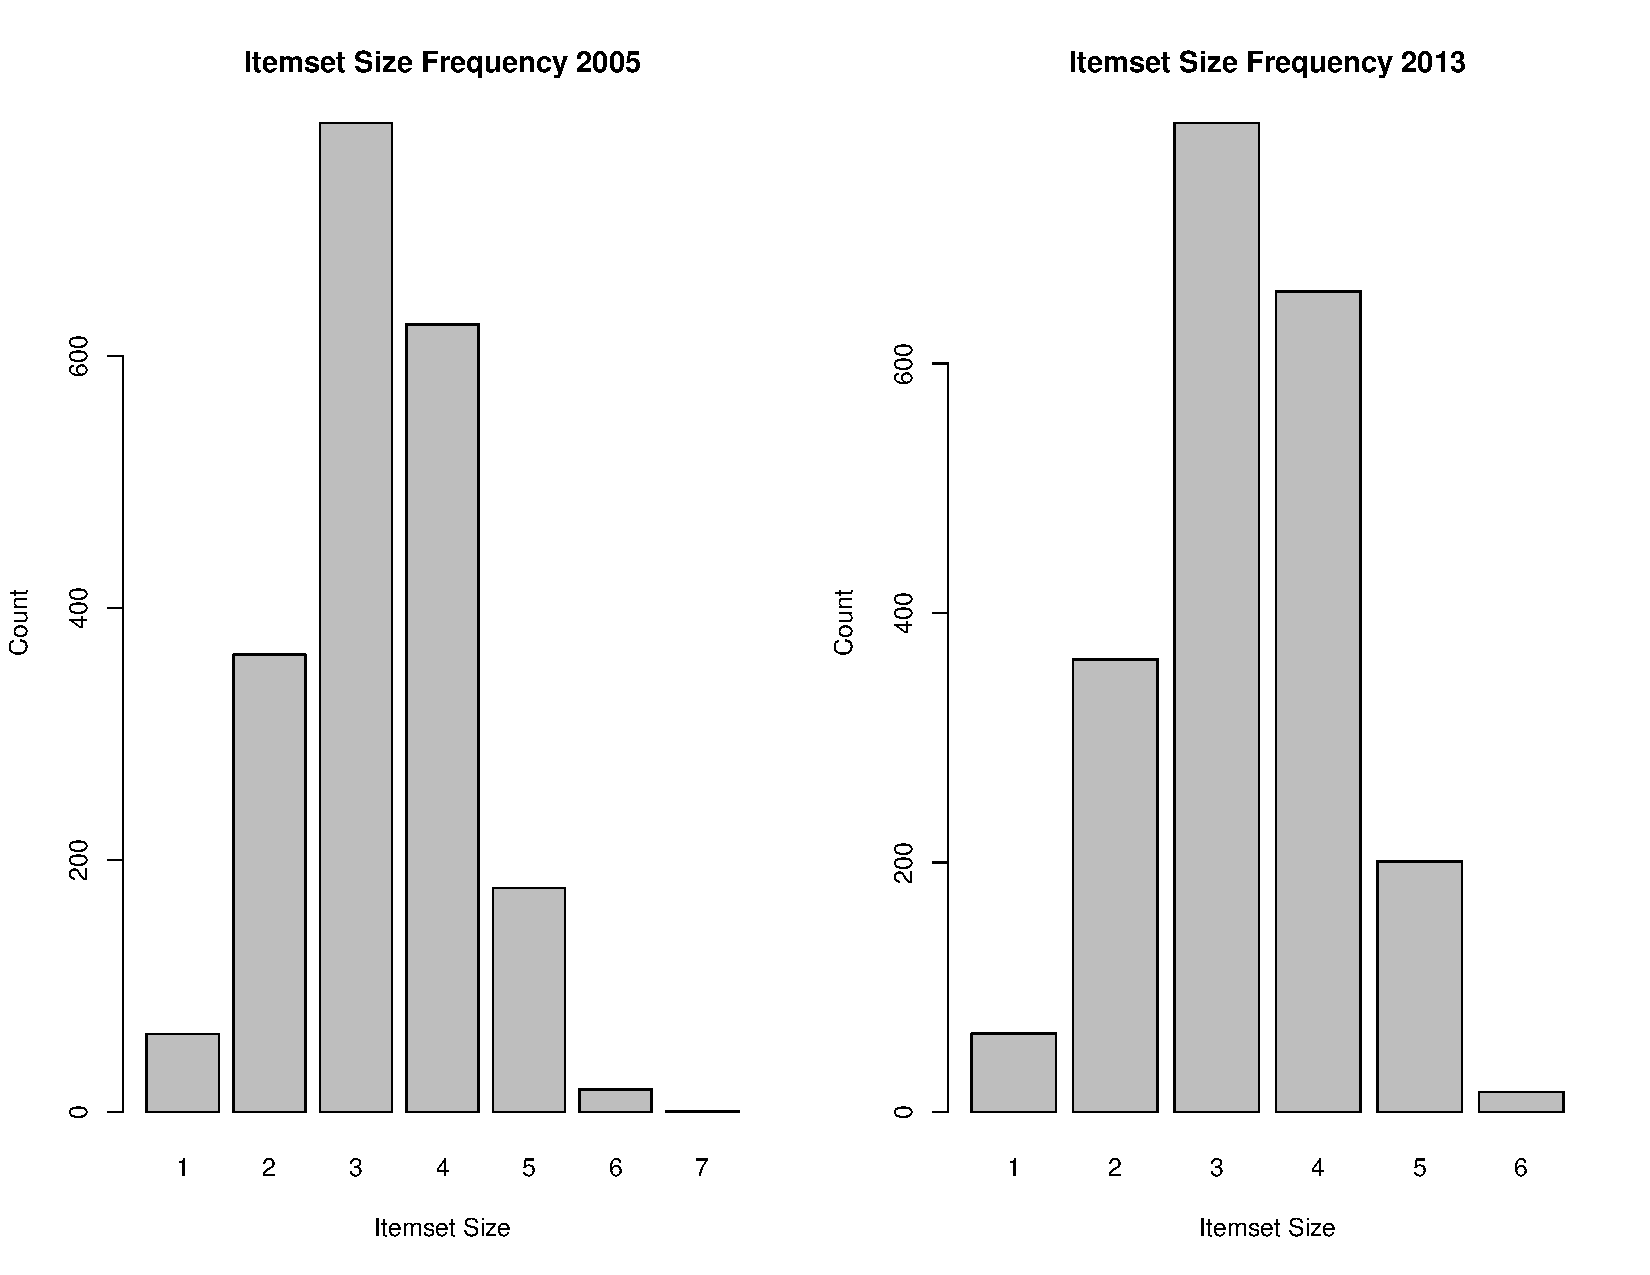
\includegraphics[scale=0.4]{./images/freq-itemset-sizes.pdf}
            \caption{The Distribution of Itemset Sizes for 2005 and 2013}
            \label{fig:1}
        \end{figure}
    \end{center}

    \begin{center}
        \begin{figure}
            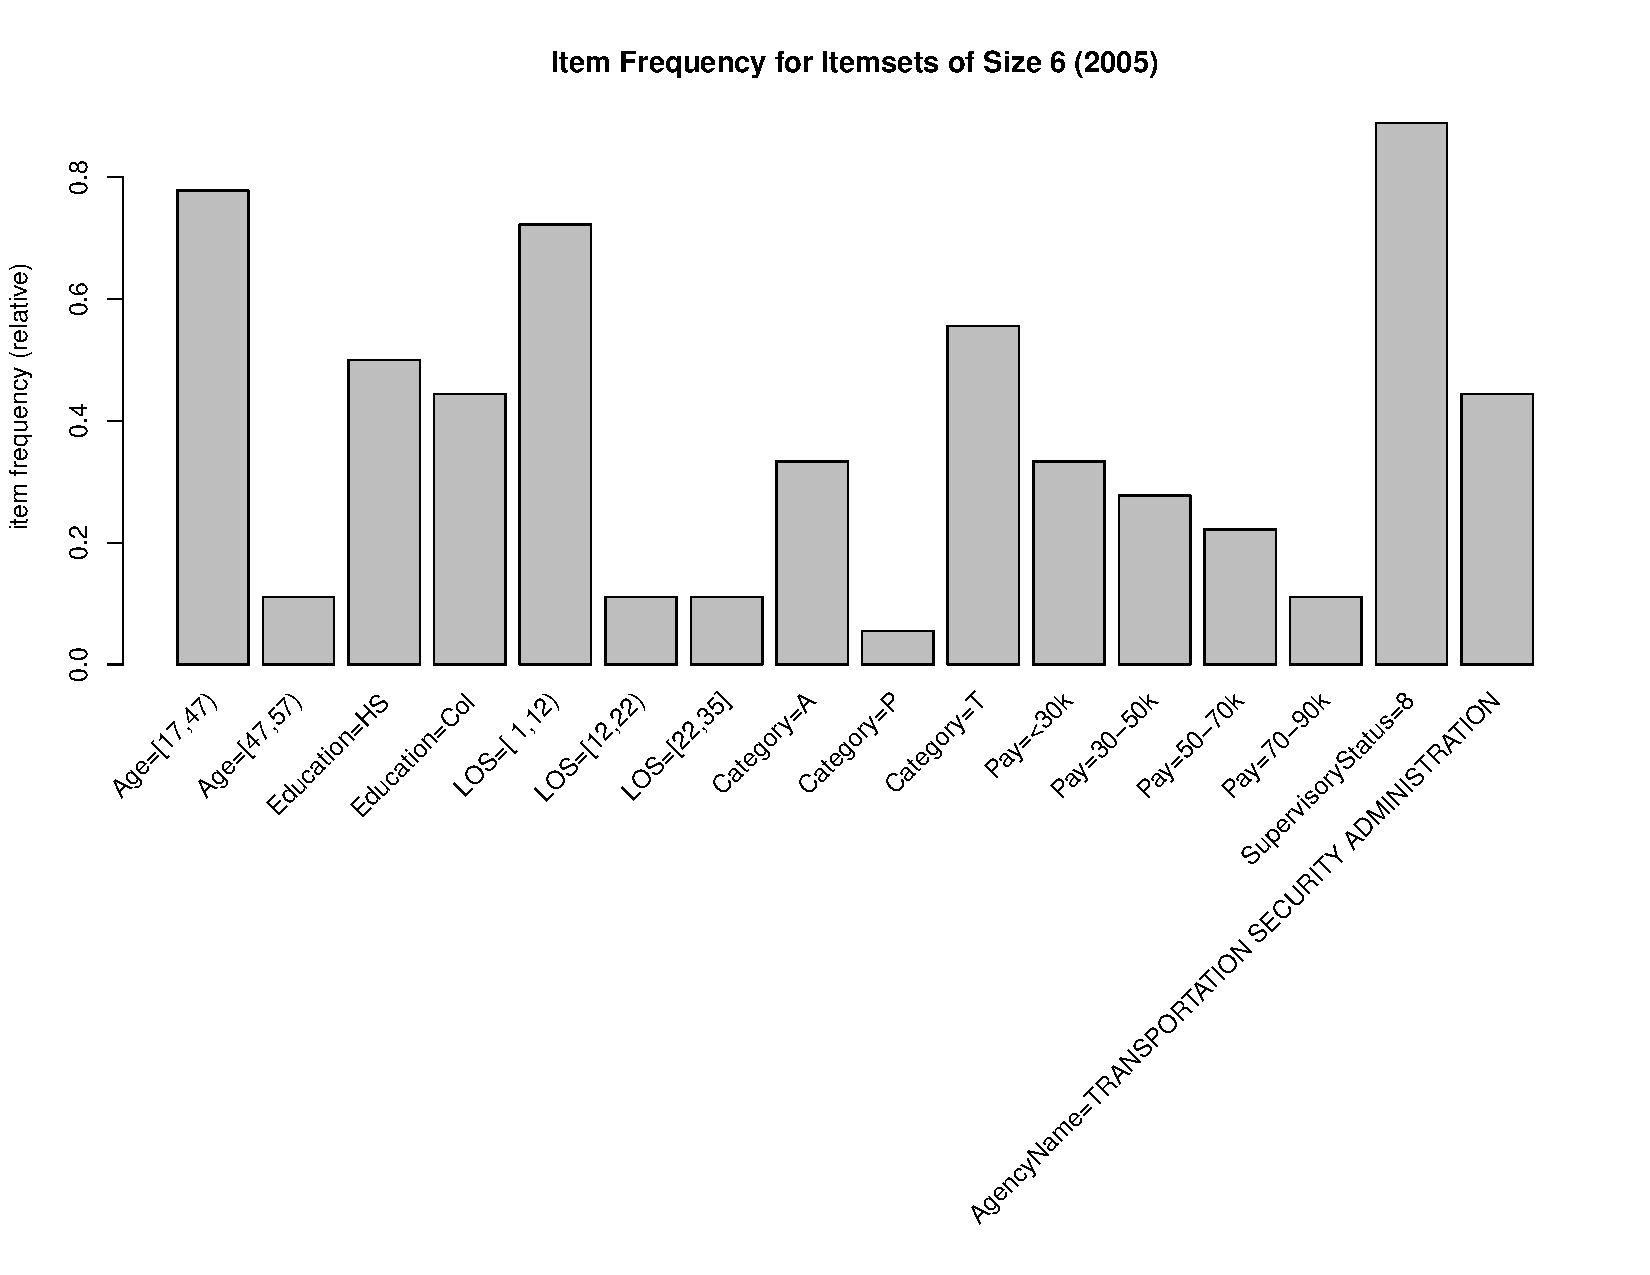
\includegraphics[scale=0.4]{./images/item-freq-2005.pdf}
            \caption{The Distribution of Items in Itemsets of Size Six for 2005}
            \label{fig:2}
        \end{figure}
    \end{center}

    \begin{center}
        \begin{figure}
            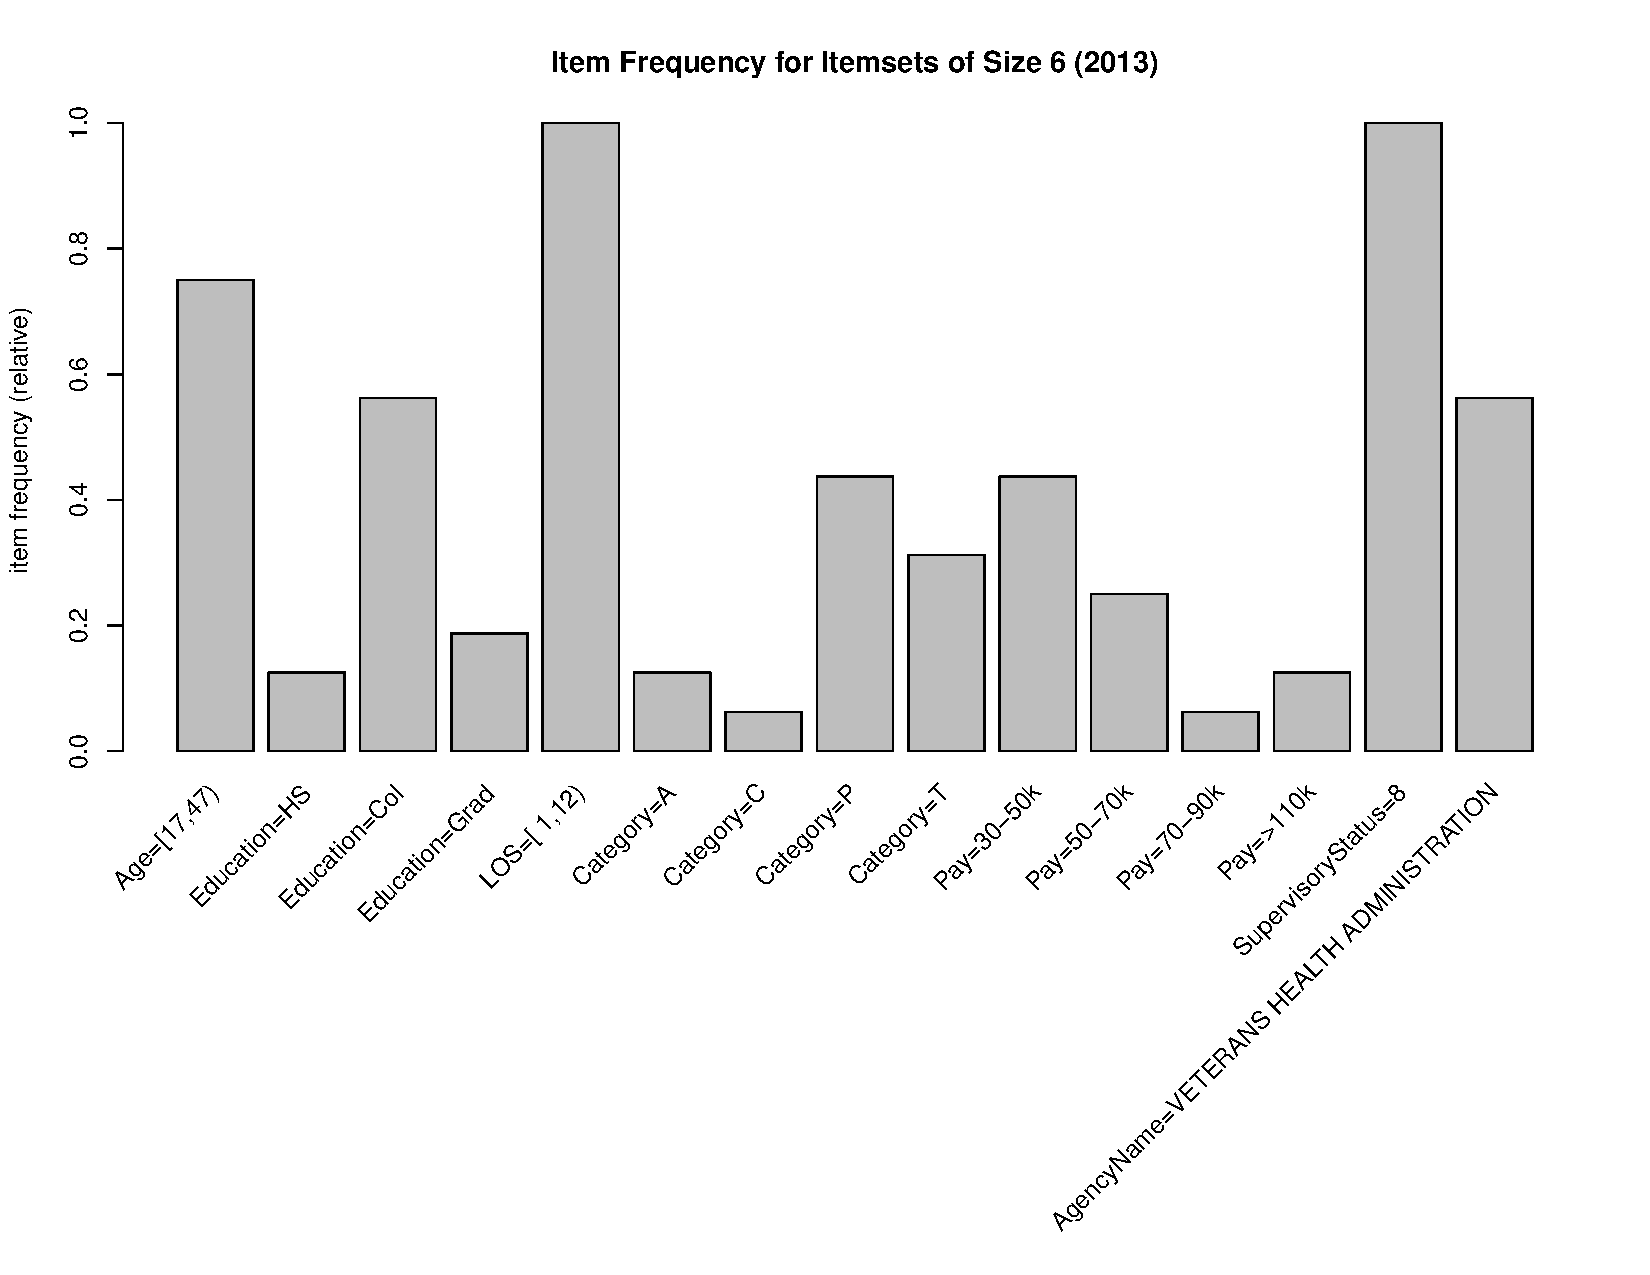
\includegraphics[scale=0.4]{./images/item-freq-2013.pdf}
            \caption{The Distribution of Items in Itemsets of Size Six for 2013}
            \label{fig:3}
        \end{figure}
    \end{center}

    \begin{center}
        \begin{table}
            \centering
            \begin{tabular}{ |c|c| }
                \hline
                \multicolumn{2}{|c|}{2005} \\
                \hline
                Itemset & Support \\
                \hline
                \{Age=[17,47),
                Education=HS,
                LOS=[1,12),
                Category=T,
                Pay=30-50k,
                SupervisoryStatus=8\} & 0.0213 \\
                \{Age=[17,47),
                Education=Col,
                LOS=[1,12),
                Category=A,
                Pay=50-70k,
                SupervisoryStatus=8\} & 0.0172 \\
                \{Age=[17,47),
                Education=Col,
                LOS=[1,12),
                Categroy=T,
                Pay=30-50k,
                SupervisoryStatus=8\} & 0.0170 \\
                \{Age=[17,47),
                Education=HS,
                LOS=[1,12),
                Category=T,
                Pay=$<$30k,
                SupervisoryStatus=8\} & 0.0165 \\
                \{Age=[17,47),
                Education=Col,
                LOS=[12,22),
                Category=A,
                Pay=70-90k,
                SupervisoryStatus=8\} & 0.0133 \\
                \hline
                \multicolumn{2}{|c|}{2013} \\
                \hline
                Itemset & Support \\
                \hline
                \{Age=[17,47),
                Education=Col,
                LOS=[1,12),
                Category=T,
                Pay=30-50k,
                SupervisoryStatus=8\} & 0.0234 \\
                \{Age=[17,47),
                Education=Col,
                LOS=[1,12),
                Category=A,
                Pay=50-70k,
                SupervisoryStatus=8\} & 0.0192 \\
                \{Age=[17,47),
                Education=HS,
                LOS=[1,12),
                Categroy=T,
                Pay=30-50k,
                SupervisoryStatus=8\} & 0.0178 \\
                \{Age=[17,47),
                Education=Col,
                LOS=[1,12),
                Category=A,
                Pay=70-90k,
                SupervisoryStatus=8\} & 0.0165 \\
                \{Age=[17,47),
                Education=Col,
                LOS=[12,22),
                Category=C,
                Pay=30-50k,
                SupervisoryStatus=8\} & 0.0133 \\
                \hline
            \end{tabular}
            \caption{Frequent Itemsets of Size Six in 2005 and 2013}
            \label{tab:5}
        \end{table}
    \end{center}

    \subsection{Closed Itemsets}
    Closed frequent itemsets are frequent itemsets that do not have a superset with a larger support value. These will show the general features that apply to large portions of the subject population. I would expect the closed frequent itemsets to express similar information to the summary statistics about the transaction data. To get the most out of the closed itemsets, I will subset the transaction data sets to a single agency to see how the structure changes between the two administrations. I will examine NASA.
    \par
    To generate this transaction data, I subsetted from the original data frames for each year and then discretized numeric attributes by frequency. This produced splits that were slightly different than when I processed the whole data frames in bulk. Only the intervals for 2013 were affected due to the increase in young employees under Obama.
    \par
    The closed frequent itemsets for each year are given in Table \ref{tab:6}. We see the ratio of supervisors increases in the later years, which is accompanied by an increase in Professional type employees. There are also more employees in professional roles who are not supervisors. This indicates that NASA developed a taller organizational structure under Obama. There is also a slight decrease in the ratio of employees who have College degrees. This is likely due to the increase in the number of Graduate level employees who joined the federal government under Obama.

    \begin{center}
        \begin{table}
            \centering
            \begin{tabular}{ |c|c| }
                \hline
                \multicolumn{2}{|c|}{2005} \\
                \hline
                Itemset & Support \\
                \hline
                \{SupervisoryStatus=8\} & 0.8606 \\
                \{Category=P\} & 0.6461 \\
                \{LOS=[1,22)\} & 0.5684 \\
                \{Category=P, SupervisoryStatus=8\} & 0.5440 \\
                \{LOS=[1,22), SupervisoryStatus=8\} & 0.5102 \\
                \{Education=Col\} & 0.4620 \\
                \{Age=[17,47)\} & 0.4407 \\
                \{Education=Col, SupervisoryStatus=8\} & 0.4088 \\
                \hline
                \multicolumn{2}{|c|}{2013} \\
                \hline
                Itemset & Support \\
                \hline
                \{SupervisoryStatus=8\} & 0.8279 \\
                \{Category=P\} & 0.6946 \\
                \{Category=P, SupervisoryStatus=8\} & 0.5693 \\
                \{Pay=$>$110k\} & 0.5620 \\
                \{Age=[17,52)\} & 0.4937 \\
                \{Category=P, Pay=$>$100k\} & 0.4646 \\
                \{Education=Col\} & 0.4388 \\
                \{Age=[17,52), SupervisoryStatus=8\} & 0.4251 \\
                \hline
            \end{tabular}
            \caption{Closed Frequent Itemsets for NASA in 2005 and 2013}
            \label{tab:6}
        \end{table}
    \end{center}

    \subsection{Maximal Itemsets}
    Itemsets are maximally frequent if none of their immediate supersets are frequent. They are the largest itemsets for the items they contain while still remaining frequent. These will show us the largest itemsets that still apply to our threshold number of employees. The top five maximally frequent itemsets by support are given in Table \ref{tab:7}.
    \par
    The most interesting maximal itemset is itemset five for 2005. This itemset indicates a large number of supervisors and managers had a high school education under Bush.

    \begin{center}
        \begin{table}
            \centering
            \begin{tabular}{ |c|c| }
                \hline
                \multicolumn{2}{|c|}{2005} \\
                \hline
                Itemset & Support \\
                \hline
                \{Age=[17,47),
                Education=Grad,
                LOS=[1,12),
                Category=P,
                SupervisoryStatus=8\} & 0.0255 \\
                \{Education=Grad,
                Category=P,
                Pay=$>$110k
                SupervisoryStatus=8\} & 0.0250 \\
                \{Education=Col,
                Category=P,
                Pay=70-90k,
                SupervisoryStatus=8\} & 0.0241 \\
                \{Age=[47,57),
                Education=HS,
                Category=T,
                Pay=30-50k,
                SupervisoryStatus=8\} & 0.0241 \\
                \{Education=HS,
                SupervisoryStatus=2\} & 0.0227 \\
                \hline
                \multicolumn{2}{|c|}{2013} \\
                \hline
                Itemset & Support \\
                \hline
                \{Age=[47,57),
                Education=Col,
                LOS=[22,35],
                Category=A,
                SupervisoryStatus=8\} & 0.0286 \\
                \{Education=HS,
                Category=A,
                Pay=70-90k,
                SupervisoryStatus=8\} & 0.0254 \\
                \{Age=[57,75],
                Education=Col,
                LOS=[22,35],
                Category=A,
                SupervisoryStatus=8\} & 0.0234 \\
                \{Age=[17,47),
                Education=Col,
                LOS=[1,12),
                Category=T,
                Pay=30-50k,
                SupervisoryStatus=8\} & 0.0234 \\
                \{Age=[17,47),
                Education=Col,
                LOS=[12,22),
                Category=A,
                SupervisoryStatus=8\} & 0.0233 \\
                \hline
            \end{tabular}
            \caption{Maximal Frequent Itemsets in 2005 and 2013}
            \label{tab:7}
        \end{table}
    \end{center}

    \subsection{Rules}
    Rules are itemsets where one of the items is a consequence of the others. In other words, the consequence is a prediction based on the remaining items in the itemset. I will use association rules to look for the common features of each SupervisoryStatus. In order to get an idea of the general rules that apply to the government as a whole, I will exclude rules that reference a particular agency.
    \par
    The list of rules for supervisors and general employees for each year is given in Table \ref{tab:8}. These rules are ranked by confidence.

    \begin{center}
        \begin{table}
            \centering
            \begin{tabular}{ |c|c|c| }
                \hline
                \multicolumn{3}{|c|}{2005} \\
                \hline
                Antecedents & Consequent & Confidence \\
                \hline
                \{Category=O,
                Pay=$>$110k\} & \{SupervisoryStatus=2\} & 0.9761 \\
                \{Category=B,
                Pay=50-70k,
                region=florida\} & \{SupervisoryStatus=2\} & 0.8890 \\
                \{Age=[47,57),
                LOS=[12,22),
                Category=O,
                Pay=70-90k\} & \{SupervisoryStatus=2\} & 0.8333 \\
                \{Age=[47,57),
                Education=Col,
                LOS=[12,22),
                Category=O,
                Pay=70-90k\} & \{SupervisoryStatus=2\} & 0.8287 \\
                \{Age=[47,57),
                Education=Col,
                Category=O,
                Pay=90k-110k\} & \{SupervisoryStatus=2\} & 0.8231 \\
                \{Education=Col,
                Category=O,
                Pay=90k-110k\} & \{SupervisoryStatus=2\} & 0.8079 \\
                \{Age=[47,57),
                Category=A,
                Pay=$<$30k\} & \{SupervisoryStatus=8\} & 1 \\
                \{Education=HS,
                Category=T,
                Pay=$<$30k,
                region=florida\} & \{SupervisoryStatus=8\} & 1 \\
                \{Education=HS,
                LOS=[1,12),
                Category=T,
                Pay=$<$30k,
                region=florida\} & \{SupervisoryStatus=8\} & 1 \\
                \{Age=[47,57),
                LOS=[1,12),
                Category=A,
                Pay=$<$30k\} & \{SupervisoryStatus=8\} & 1 \\
                \{Category=T,
                Pay=$<$30k,
                region=georgia\} & \{SupervisoryStatus=8\} & 1 \\
                \{LOS=[1,12),
                Category=T,
                Pay=$<$30k,
                region=georgia\} & \{SupervisoryStatus=8\} & 1 \\
                \hline
                \multicolumn{3}{|c|}{2013} \\
                \hline
                Itemset & Support \\
                \hline
                \{Age=[47,57),
                Education=Col,
                LOS=[22,35],
                Category=O,
                Pay=$>$110k\} & \{SupervisoryStatus=2\} & 0.9289 \\
                \{Education=Col,
                LOS=[22,35],
                Category=O,
                Pay=$>$110k\} & \{SupervisoryStatus=2\} & 0.9220 \\
                \{Age=[47,57),
                LOS=[22,35],
                Category=O,
                Pay=$>$110k\} & \{SupervisoryStatus=2\} & 0.9168 \\
                \{LOS=[22,35],
                Category=O,
                Pay=$>$110k\} & \{SupervisoryStatus=2\} & 0.8949 \\
                \{Age=[17,47),
                Education=HS,
                LOS=[12,22),
                Category=O,
                Pay=90k-110k\} & \{SupervisoryStatus=2\} & 0.8828 \\
                \{Age=[47,57),
                Education=Col,
                Category=O,
                Pay=$>$110k\} & \{SupervisoryStatus=2\} & 0.8821 \\
                \{Age=[57,75],
                Category=T,
                Pay=$<$30k\} & \{SupervisoryStatus=2\} & 1 \\
                \{Education=Doc,
                Pay=50-70k,
                region=maryland\} & \{SupervisoryStatus=2\} & 1 \\
                \{Education=Doc,
                LOS=[1,12),
                Pay=50-70k,
                region=maryland\} & \{SupervisoryStatus=2\} & 1 \\
                \{Education=Doc,
                Category=P,
                Pay=50-70k,
                region=maryland\} & \{SupervisoryStatus=2\} & 1 \\
                \{Age=[57,75],
                LOS=[1,12),
                Category=T,
                Pay=$<$30k\} & \{SupervisoryStatus=2\} & 1 \\
                \{Education=Doc,
                LOS=[1,12),
                Category=P,
                Pay=50-70k,
                region=maryland\} & \{SupervisoryStatus=2\} & 1 \\
                \hline
            \end{tabular}
            \caption{Top SupervisoryStatus Rules for 2005 and 2013}
            \label{tab:8}
        \end{table}
    \end{center}


\section{Evaluation}

\begin{thebibliography}{10}
    \bibitem{proj1}
    Jake Carlson
    \textit{CSE 5331 - Data Mining Project 1}
    \texttt{https://github.com/jakecarlson1/data-mining-projects/blob/master/}
    \texttt{project-1/report/carlson-project-1.pdf}

    \bibitem{proj2}
    Jake Carlson
    \textit{CSE 5331 - Data Mining Project 2}
    \texttt{https://github.com/jakecarlson1/data-mining-projects/blob/master/}
    \texttt{project-2/report/carlson-project-2.pdf}

\end{thebibliography}

\end{document}
